%%%%%%%%%%%%%%%%%%%% author.tex %%%%%%%%%%%%%%%%%%%%%%%%%%%%%%%%%%%
%
% sample root file for your 'contribution' to a contributed volume
%
% Use this file as a template for your own input.
%
%%%%%%%%%%%%%%%% Springer %%%%%%%%%%%%%%%%%%%%%%%%%%%%%%%%%%


% RECOMMENDED %%%%%%%%%%%%%%%%%%%%%%%%%%%%%%%%%%%%%%%%%%%%%%%%%%%
\documentclass[graybox]{svmult}

% choose options for [] as required from the list
% in the Reference Guide

%\usepackage{type1cm}        % activate if the above 3 fonts are
                            % not available on your system
%
\usepackage{makeidx}         % allows index generation
% \usepackage{graphicx}        % standard LaTeX graphics tool  %%% modified by Sakagami,H. 19/10/10
\usepackage[dvipdfmx]{graphicx}   
                             % when including figure files
\usepackage{multicol}        % used for the two-column index
\usepackage[bottom]{footmisc}% places footnotes at page bottom


\usepackage{newtxtext}       % 
\usepackage{newtxmath}       % selects Times Roman as basic font

\usepackage{listings} %%% inserted by Sakagami,H. 19/10/10
\lstset{language=[08]Fortran, basicstyle=\ttfamily\footnotesize, numbers=left, numberstyle={\ttfamily\small}, frame=single}

% see the list of further useful packages
% in the Reference Guide

\makeindex             % used for the subject index
                       % please use the style svind.ist with
                       % your makeindex program

%%%%%%%%%%%%%%%%%%%%%%%%%%%%%%%%%%%%%%%%%%%%%%%%%%%%%%%%%%%%%%%%%%%%%%%%%%%%%%%%%%%%%%%%%

\begin{document}

\title*{Three-dimensional Fluid Code with XcalableMP}
% Use \titlerunning{Short Title} for an abbreviated version of
% your contribution title if the original one is too long
\author{Hitoshi Sakagami}
% Use \authorrunning{Short Title} for an abbreviated version of
% your contribution title if the original one is too long
\institute{Hitoshi Sakagami \at National Institute for Fusion Science, 322-6 Oroshi-cho, Toki 509-5292, Japan, \email{sakagami.hitoshi@nifs.ac.jp}
}
%
% Use the package 'url.sty' to avoid
% problems with special characters
% used in your e-mail or web address
%
\maketitle

\abstract{In order to adapt parallel computers to general convenient tools for computational scientists, a high-level and easy-to-use portable parallel programming paradigm is mandatory. XcalableMP, which is proposed by the XcalableMP Specification Working Group, is a directive-based language extension for Fortran and C to easily describe parallelization in programs for distributed memory parallel computers. The Omni XcalableMP compiler, which is provided as a reference XcalableMP compiler, is currently implemented as a source-to-source translator. It converts XcalableMP programs to standard MPI programs, which can be easily compiled by the native Fortran compiler and executed on most of parallel computers. A three-dimensional Eulerian fluid code written in Fortran is parallelized by XcalableMP using two different programming models with the ordinary domain decomposition method, and its performances are measured on the K computer. Programs converted by the Omni XcalableMP compiler prevent native Fortran compiler optimizations and show lower performance than that of hand-coded MPI programs. Finally almost the same performances are obtained by using specific compiler options of the native Fortran compiler in the case of a global-view programming model, but performance degradation is not improved by specifying any native compiler options when the code is parallelized by a local-view programming model.}

\section{Introduction}
Computational scientists usually want to concentrate their attention on their essential research. Parallel programming is never an objective for them even if computational powers of parallel computers are necessary to advance their subjects, and this dilemma is annoying them. In order to adapt the parallel computer from a special kind of machines to general convenient tools for computational scientists, a high-level and easy-to-use portable parallel programming paradigm is mandatory. XcalableMP (XMP) \cite{XMP}, which is proposed by the XcalableMP Specification Working Group, is directive-based language extensions for Fortran and C to easily describe parallelization in programs for distributed memory parallel computers. The XMP/F compiler \cite{Omni}, which is provided as a reference XMP Fortran compiler, is currently implemented as a source-to-source translator. It converts XMP Fortran programs to standard MPI Fortran programs, which can be easily compiled by the native Fortran compiler and executed on most of parallel computers.

XMP supports typical data/task parallelization methods with simple directives under a ``global-view'' programming model, which is partially based on experiences of High Performance Fortran \cite{HPF,Ken} and Fujitsu XPF (VPP FORTRAN) \cite{Zhang}. XMP also supports PGAS (Partitioned Global Address Space) features like Coarray Fortran \cite{CAF} as a ``local-view'' programming model. In addition, combinations of XMP and OpenMP directives are consistently maintained by the XMP/F compiler. An essential design principle of XMP is ``performance awareness'', which means that all communications or synchronizations are taken by explicit directives or Coarray statements and no implicit actions are taken.

First, we used XMP Fortran to parallelize the code using the global-view programming model, and measured its performance on the K computer. We found that programs converted by the XMP/F compiler prevent optimizations by the native Fortran compiler and show lower performance than that by hand-coded MPI programs, but finally almost the same performances are obtained by using specific compiler options of the native Fortran compiler. Next we parallelized the code using the local-view programming model, and also measured its performance on the K computer. We found that translated programs prevent optimizations by the native Fortran compiler and show lower performance than that of the global-view programming model programs. This degradation can not be solved by simply specifying native compiler options at this moment, and improvements of the XMP/F compiler are expected.

\section{Global-view Programming Model}
IMPACT-3D is a three-dimensional Eulerian fluid code written in Fortran and it performs compressible and inviscid fluid computation to simulate convergent asymmetric flows related to laser fusion \cite{SC02}. A Cartesian coordinate system is employed and an explicit 5-point stencil in one direction is used in IMPACT-3D with uniform grid spacing. So it is easy to parallelize the code with the ordinary domain decomposition method. Communications between neighboring subdomains are needed to exchange boundary data. 

As the global-view programming model is a directive oriented approach, programs can be incrementally parallelized and different parallelization methods can be easily tried. Although IMPACT-3D is actually parallelized by three different methods, original source codes are completely same and there are a few directive differences among three methods.

\subsection{Domain Decomposition Methods}
The code is parallelized by three different domain decomposition methods, namely the domain is divided in (a) only Z direction, (b) both Y and Z directions and (c) all of X, Y and Z directions, which are shown in Fig. \ref{fig6-1}. 

\begin{figure}[h]
%\sidecaption
\begin{center}
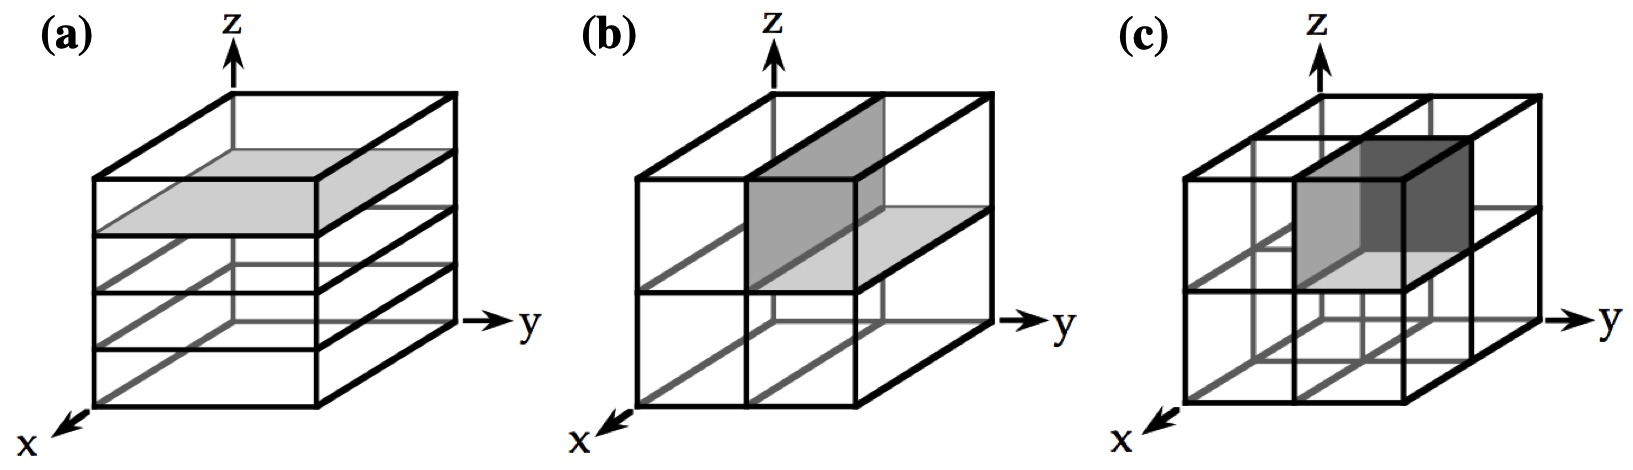
\includegraphics[width=11.5cm,bb=0 0 1633 470]{fig6-1.png}
\end{center}
\caption{IMPACT-3D is parallelized by three different domain decomposition methods. The domain is divided in (a) only Z direction, (b) both Y and Z directions and (c) all of X, Y and Z directions.}
\label{fig6-1} 
\end{figure}

Assume {\it LX, LY} and {\it LZ} are system mesh sizes of the code in X, Y and Z directions, and {\it NX, NY} and {\it NZ} are division numbers in X, Y and Z directions, respectively. In the case of only Z domain decomposition method, total amount of communicated data per domain is proportional to $LX \cdot LY$, which is not depended on any division numbers, and communication occurs twice per time step. On the other hand, data proportional to $(LX \cdot LY) \div NY$ must be communicated twice and that of ($LZ \cdot LX) \div NZ$ is also communicated twice per domain per time step in both Y and Z domain decomposition method. In the case of all of X, Y and Z domain decomposition method, data proportional to $(LX \cdot LY) \div (NX \cdot NY)$,  $(LZ \cdot LX) \div (NZ \cdot NX)$ and $(LY \cdot LZ) \div (NY \cdot NZ)$ must be communicated per domain per time step twice, twice and three times, respectively. Thus total communication costs in three different domain decomposition methods are depended on a trade-off between latency and speed. Additional communication is one reduction operation to obtain a maximum scalar value in whole simulation system.

A node array that corresponds with physical compute units in parallel computer is defined by {\it node} directive, three-dimensional Fortran arrays are decomposed with {\it template, distribute} and {\it align} directives, corresponding DO loops are parallelized by {\it loop} directive and communications between neighboring subdomains are implemented by {\it shadow} and {\it reflect} directives. The code can be parallelized by using the ``global-view'' programming model directives only. Typical XMP Fortran programs are shown for each decomposition method,  in Listing \ref{onlyz} for only Z direction, Listing \ref{bothyz} for both Y and Z directions and Listing \ref{allxyz} for all of X, Y and Z directions.
{\it lx, ly, lz} are Fortran array size of first, second, third dimension, and {\it nx, ny, nz} are a number of division in X, Y, Z direction, respectively. These are also variable names in the program shown in Listings.

The code is also hand-coded with MPI using the same domain decomposition methods to compare performances.

\begin{lstlisting}[caption=Typical XMP programs using the global-view programming model for only Z domain decomposition method., label=onlyz]
integer parameter :: lx=..., ly=..., lz=...
integer parameter :: nz=...
!$XMP NODES proc(nz)
!$XMP TEMPLATE t(lx,ly,lz)
!$XMP DISTRIBUTE t(*,*,BLOCK) ONTO proc
real*8 :: physval(6,lx,ly,lz)
real*8 :: ram
!$XMP ALIGN (*,*,*,k) WITH t(*,*,k) :: physval
!$XMP SHADOW (0,0,0,1) :: physval 
...
!$XMP LOOP (iz) ON t(*,*,iz)
!$OMP PARALLEL DO PRIVATE(iy,ix)
do iz = 1, lz
 do iy = 1, ly
  do ix = 2, lx-1 
   ...
   physval(..,ix,iy,iz) = ... &
      physval(..,ix-1,iy,iz) ... physval(..,ix+1,iy,iz)
   ...
...
!$XMP LOOP (iz) ON t(*,*,iz)
!$OMP PARALLEL DO PRIVATE(iy,ix)
do iz = 1, lz
 do iy = 2, ly-1
  do ix = 1, lx 
   ...
   physval(..,ix,iy,iz) = ... &
      physval(..,ix,iy-1,iz) ... physval(..,ix,iy+1,iz)
   ...
...
!$XMP REFLECT (physval) 
!$XMP LOOP (iz) ON t(*,*,iz)
!$OMP PARALLEL DO PRIVATE(iy,ix)
do iz = 2, lz-1
 do iy = 1, ly
  do ix = 1, lx 
   ...
   physval(..,ix,iy,iz) = ... &
      physval(..,ix,iy,iz-1) ... physval(..,ix,iy,iz+1)
   ...
...
!$XMP LOOP (iz) ON t(*,*,iz) REDUCTION(max:ram)
!$OMP PARALLEL DO REDUCTION(max:ram) PRIVATE(iy,ix)
do iz = 1, lz
 do iy = 1, ly
  do ix = 1, lx 
   ram = max( ram, ... ) 
\end{lstlisting}

\begin{lstlisting}[caption=Typical XMP programs using the global-view programming model for both Y and Z domain decomposition method., label=bothyz]
integer parameter :: lx=..., ly=..., lz=...
integer parameter :: ny=..., nz=...
!$XMP NODES proc(ny,nz) 
!$XMP TEMPLATE t(lx,ly,lz)
!$XMP DISTRIBUTE t(*,BLOCK,BLOCK) ONTO proc
real*8 :: physval(6,lx,ly,lz)
real*8 :: ram
!$XMP ALIGN (*,*,j,k) WITH t(*,j,k) :: physval 
!$XMP SHADOW (0,0,1,1) :: physval 
...
!$XMP LOOP (iy,iz) ON t(*,iy,iz)
!$OMP PARALLEL DO PRIVATE(iy,ix)
do iz = 1, lz
 do iy = 1, ly
  do ix = 2, lx-1 
   ...
   physval(..,ix,iy,iz) = ... &
      physval(..,ix-1,iy,iz) ... physval(..,ix+1,iy,iz)
   ...
...
!$XMP REFLECT (physval) width(0,0,1,0) 
!$XMP LOOP (iy,iz) ON t(*,iy,iz)
!$OMP PARALLEL DO PRIVATE(iy,ix)
do iz = 1, lz
 do iy = 2, ly-1
  do ix = 1, lx 
   ...
   physval(..,ix,iy,iz) = ... &
      physval(..,ix,iy-1,iz) ... physval(..,ix,iy+1,iz)
   ...
...
!$XMP REFLECT (physval) width(0,0,0,1) 
!$XMP LOOP (iy,iz) ON t(*,iy,iz)
!$OMP PARALLEL DO PRIVATE(iy,ix)
do iz = 2, lz-1
 do iy = 1, ly
  do ix = 1, lx 
   ...
   physval(..,ix,iy,iz) = ... &
      physval(..,ix,iy,iz-1) ... physval(..,ix,iy,iz+1)
   ...
...
!$XMP LOOP (iy,iz) ON t(*,iy,iz) REDUCTION(max:ram)
!$OMP PARALLEL DO REDUCTION(max:ram) PRIVATE(iy,ix)
do iz = 1, lz
 do iy = 1, ly
  do ix = 1, lx 
   ram = max( ram, ... ) 
\end{lstlisting}

\begin{lstlisting}[caption={Typical XMP programs using the global-view programming model for all of X, Y and Z domain decomposition method.}, label=allxyz]
integer parameter :: lx=..., ly=..., lz=...
integer parameter :: nx=..., ny=..., nz=...
!$XMP NODES proc(nx,ny,nz)
!$XMP TEMPLATE t(lx,ly,lz)
!$XMP DISTRIBUTE t(BLOCK,BLOCK,BLOCK) ONTO proc
real*8 :: physval(6,lx,ly,lz)
real*8 :: ram
!$XMP ALIGN (*,i,j,k) WITH t(i,j,k) :: physval
!$XMP SHADOW (0,1,1,1) :: physval 
...
!$XMP REFLECT (physval) width(0,1,0,0) 
!$XMP LOOP (ix,iy,iz) ON t(ix,iy,iz)
!$OMP PARALLEL DO PRIVATE(iy,ix)
do iz = 1, lz
 do iy = 1, ly
  do ix = 2, lx-1 
   ...
   physval(..,ix,iy,iz) = ... &
      physval(..,ix-1,iy,iz) ... physval(..,ix+1,iy,iz)
   ...
...
!$XMP REFLECT (physval) width(0,0,1,0) 
!$XMP LOOP (ix,iy,iz) ON t(ix,iy,iz)
!$OMP PARALLEL DO PRIVATE(iy,ix)
do iz = 1, lz
 do iy = 2, ly-1
  do ix = 1, lx 
   ...
   physval(..,ix,iy,iz) = ... &
      physval(..,ix,iy-1,iz) ... physval(..,ix,iy+1,iz)
   ...
...
!$XMP REFLECT (physval) width(0,0,0,1) 
!$XMP LOOP (ix,iy,iz) ON t(ix,iy,iz)
!$OMP PARALLEL DO PRIVATE(iy,ix)
do iz = 2, lz-1
 do iy = 1, ly
  do ix = 1, lx 
   ...
   physval(..,ix,iy,iz) = ... &
      physval(..,ix,iy,iz-1) ... physval(..,ix,iy,iz+1)
   ...
...
!$XMP LOOP (ix,iy,iz) ON t(ix,iy,iz) REDUCTION(max:ram)
!$OMP PARALLEL DO REDUCTION(max:ram) PRIVATE(iy,ix)
do iz = 1, lz
 do iy = 1, ly
  do ix = 1, lx 
   ram = max( ram, ... ) 
\end{lstlisting}

\subsection{Performance on the K Computer}
As one node consists of 8 cores in the K computer, one MPI process is dispatched onto each node and each process performs computations with 8 threads. We run both XMP and MPI codes with three different decomposition methods and evaluate the weak scaling on the K computer using Omni XcalableMP 0.7.0 and Fujitsu Fortran K-1.2.0.15. A number of cores for execution and corresponding simulation parameters are summarized in Table \ref{tab6-1}.

Performance are measured by a hardware monitor installed on the K computer, and MFLOPS/PEAK, Memory throughput/PEAK and SIMD execution usage are obtained.

\begin{table}[h]
\caption{Simulation Parameters for Global-view Programming Model}
\label{tab6-1}
\begin{tabular}{p{2cm}p{2cm}p{1.5cm}p{1cm}p{1.5cm}p{1cm}p{1cm}p{1cm}}
\hline\noalign{\smallskip}
\#core & {\it lx=ly=lz} & Only Z & \multicolumn{2}{l}{both Y and Z}  & \multicolumn{3}{l}{all of X, Y and Z} \\
\cline{3-8}
 & & {\it nz} &  {\it ny} & {\it nz} & {\it nx} & {\it ny} & {\it nz} \\
\noalign{\smallskip}\svhline\noalign{\smallskip}
256 & 1024 & 32 & 8 & 4 & 4 & 4 & 2 \\
2048 & 2048 & 256 & 16 & 16 & 8 & 8 & 4 \\
16384 & 4096 & & 64 & 32 & 16 & 16 & 8 \\
131072 & 8192 & & 128 & 128 & 32 & 32 & 16  \\
\noalign{\smallskip}\hline\noalign{\smallskip}
\end{tabular}
\end{table}

\subsubsection{Comparison with Hand-coded MPI Program}
MFLOPS/PEAK values for all 6 cases, namely (MPI, XMP) x (only Z, both Y and Z, all of X, Y and Z) are shown in Fig. \ref{fig6-2}.

\begin{figure}[h]
%\sidecaption
\begin{center}
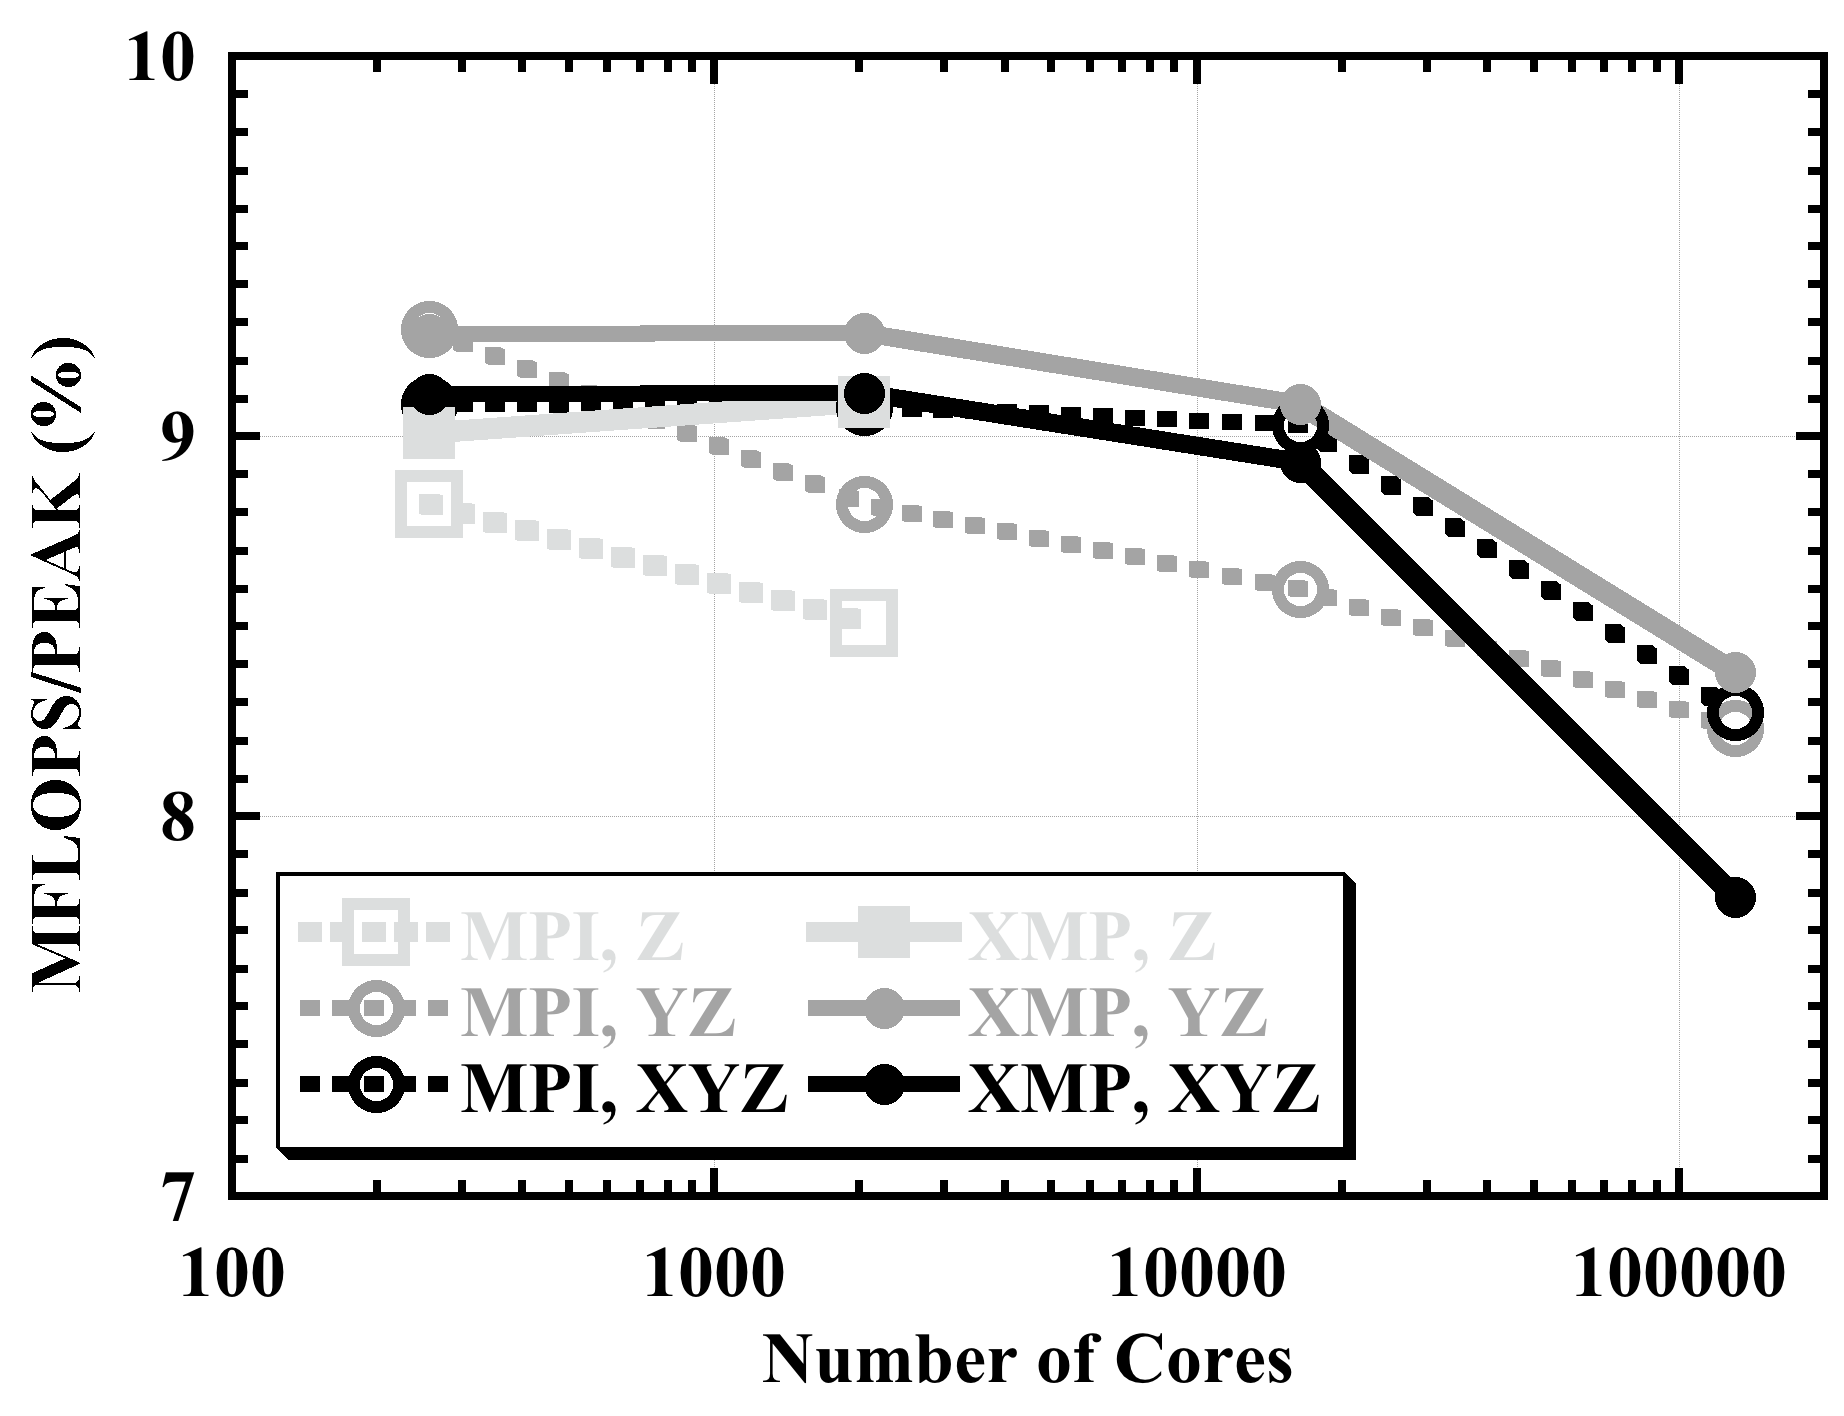
\includegraphics[width=8.5cm,bb=0 0 459 352]{fig6-2.png}
\end{center}
\caption{MFLOPS/PEAK measured by the hardware monitor installed on the K computer. Solid and dash lines indicate performances of  XMP and MPI codes, respectively. Colors of black, gray and light gray indicate only Z domain decomposition, both Y and Z domain decomposition and all of X, Y and Z domain decomposition methods, respectively.}
\label{fig6-2} 
\end{figure}

Performance of XMP codes is as same as those of MPI codes, and small differences among three decomposition methods are found. But we can get only 8\textasciitilde 9\% of peak performance of the K computer. From the hardware monitor, we found that SIMD execution usage was less than 5\% in all cases, and this could degrade the performance. Most cost intensive DO loops in IMPACT-3D include IF statements, which are needed to correctly treat extremely slow fluid velocity regardless of XMP and MPI codes, and the IF statement interrupts the native Fortran compiler to generate SIMD instructions inside the DO loop. Thus relatively low performance is obtained. 

\subsubsection{Optimization for SIMD}
As the true rate of the IF statement is nearly 100\% in IMPACT-3D, speculative execution of SIMD instruction causes almost no overhead. So forcing the compiler to generate the SIMD instructions could be useful to enhance the performance, and it can be done with {\it simd=2} compiler option. All codes are recompiled with that option and rerun. SIMD execution usage increases up to around 50\% in all cases, and we can expect performance improvement. MFLOPS/PEAK values for all cases are shown in Fig. \ref{fig6-3}.

\begin{figure}[h]
%\sidecaption
\begin{center}
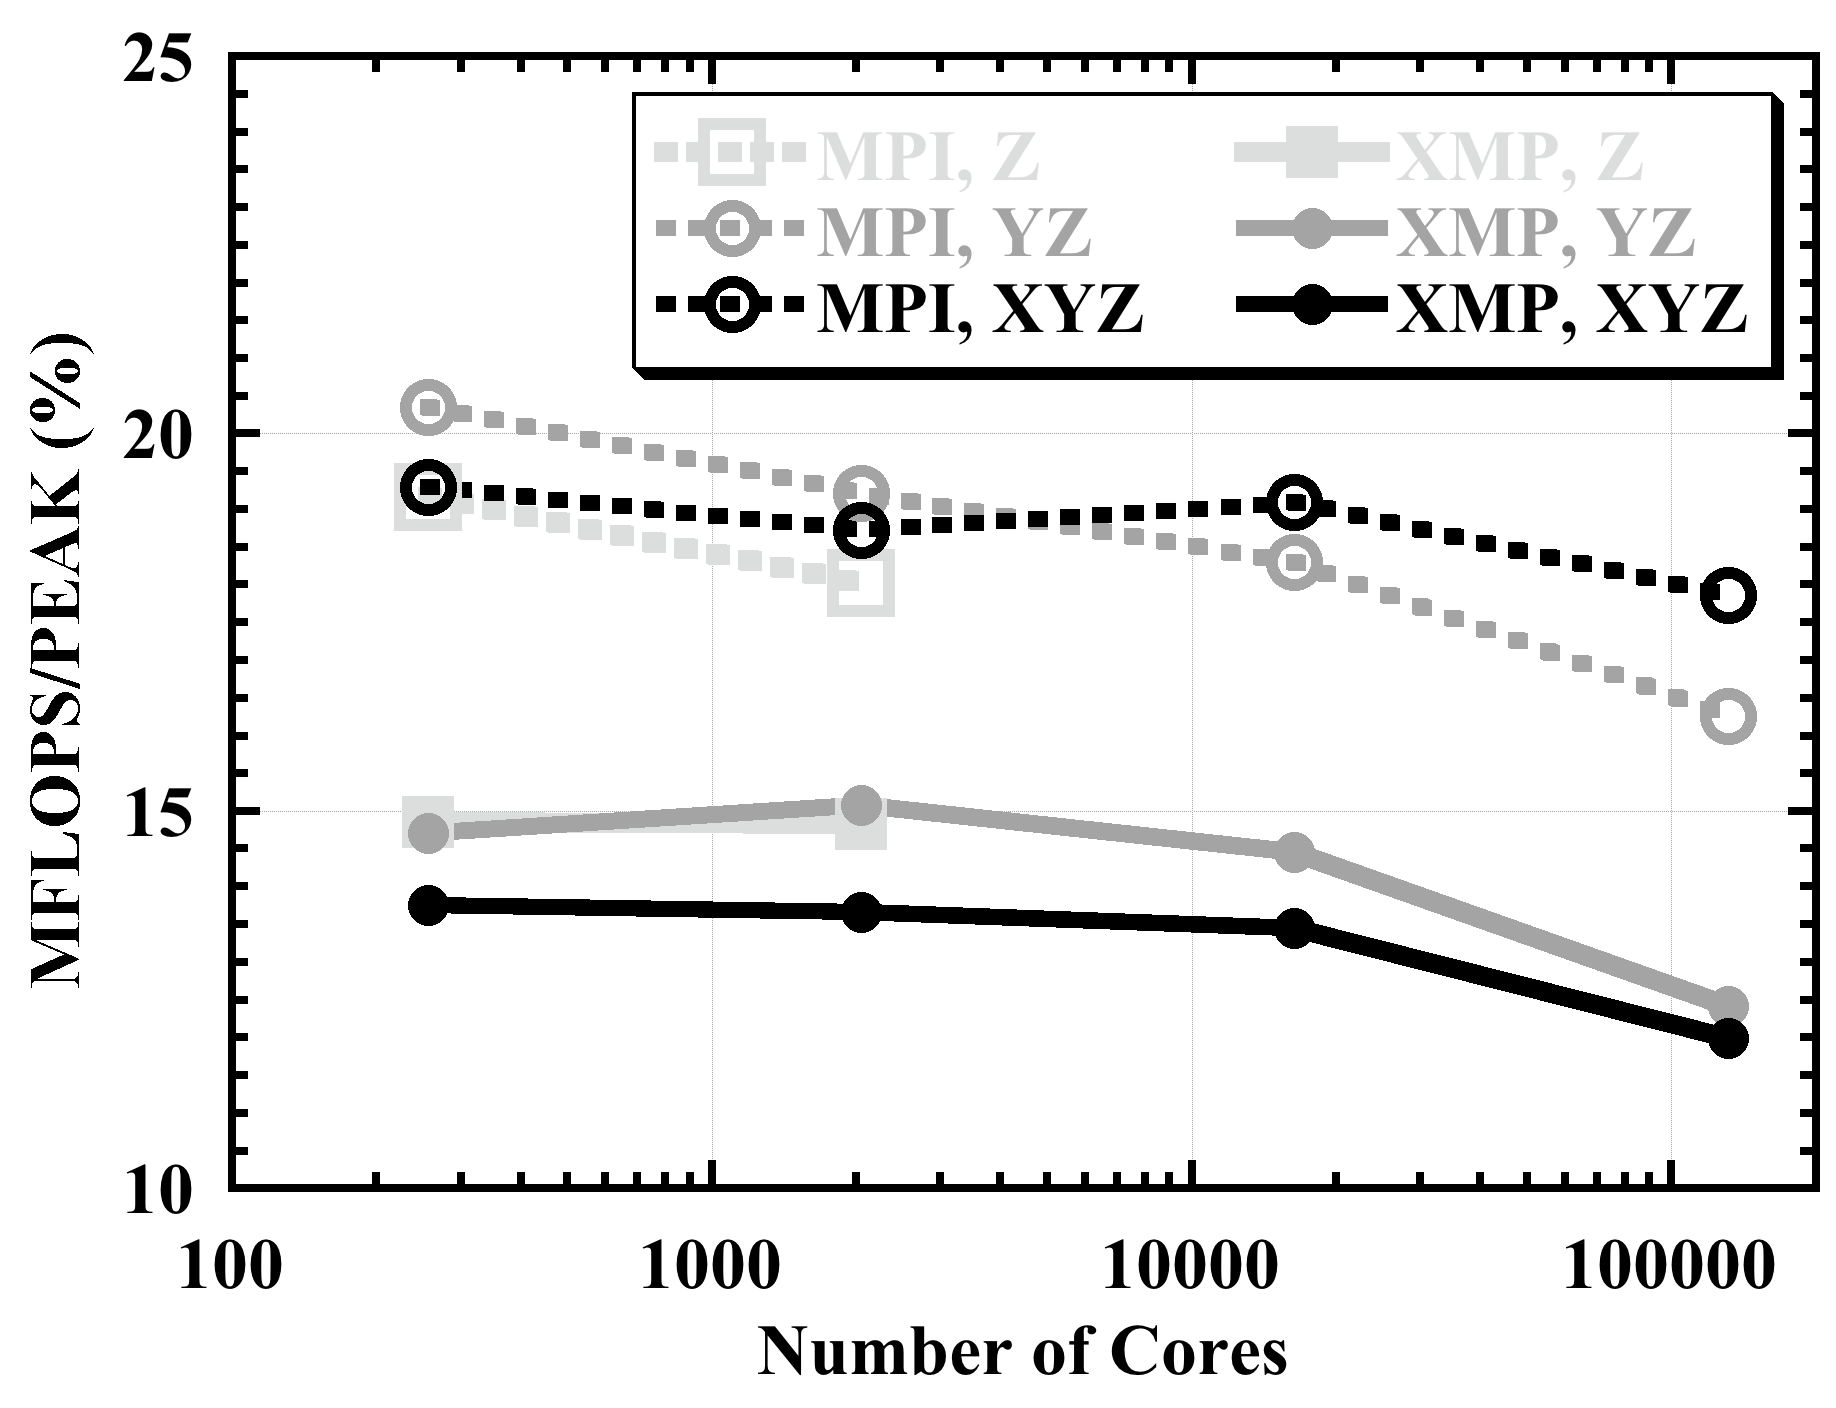
\includegraphics[width=8.5cm,bb=0 0 459 352]{fig6-3.png}
\end{center}
\caption{MFLOPS/PEAK measured by the hardware monitor installed on the K computer with SIMD optimization by {\it simd=2} compiler option. Solid and dash lines indicate performances of  XMP and MPI codes, respectively. Colors of black, gray and light gray indicate only Z domain decomposition, both Y and Z domain decomposition and all of X, Y and Z domain decomposition methods, respectively.}
\label{fig6-3} 
\end{figure}

Small differences among three decomposition methods are also found with this compiler option. MPI code performance is improved and we can get up to 20\% of the peak performance. XMP code performance is also improved, but these are below 15\% even MPI and XMP code performance is almost same without {\it simd=2} option. According to compiler diagnostic of the native Fortran compiler, the software pipelining is adopted for cost intensive DO loops in the MPI code, but it is not applied for the source code converted by the XMP/F compiler from the XMP code. As the XMP/F compiler converts a simple DO statement of ``do i = is, ie'' to more general form ``do i1 = xmp\_s1, xmp\_e1, xmp\_d1'' and the native Fortran compiler can not optimize the DO loop because do increment is given by a variable and it is unknown at compilation time. So we improved the XMP/F compiler to generate ``do i1 = xmp\_s1, xmp\_e1, 1'' form when the do increment is not given and supposed to be one in the XMP code. As a result, the software pipelining is also adopted for cost intensive DO loops converted by the XMP/F compiler, but no performance improvement is obtained. Although Memory throughput/PEAK values of MPI codes are 55\%, those of XMP codes are only 37\% and this low memory throughput is one of candidates for low sustained performance. 

\subsubsection{Optimization for Allocatable Arrays}
In the converted code by the XMP/F compiler, all Fortran arrays are treated as allocatable arrays even the original code uses static arrays. The allocatable array prevents the native Fortran compiler from optimizing the DO loop with prefetch instructions because the array size cannot be determined at compilation time, and it could cause low memory throughput. All Fortran arrays in the hand-coded MPI code for XYZ decomposition are just replaced by allocatable arrays and we check a performance difference. Performance of the MPI code are shown in Fig. \ref{fig6-4} for static arrays (light gray dash) and allocatable arrays (gray dash).

\begin{figure}[h]
%\sidecaption
\begin{center}
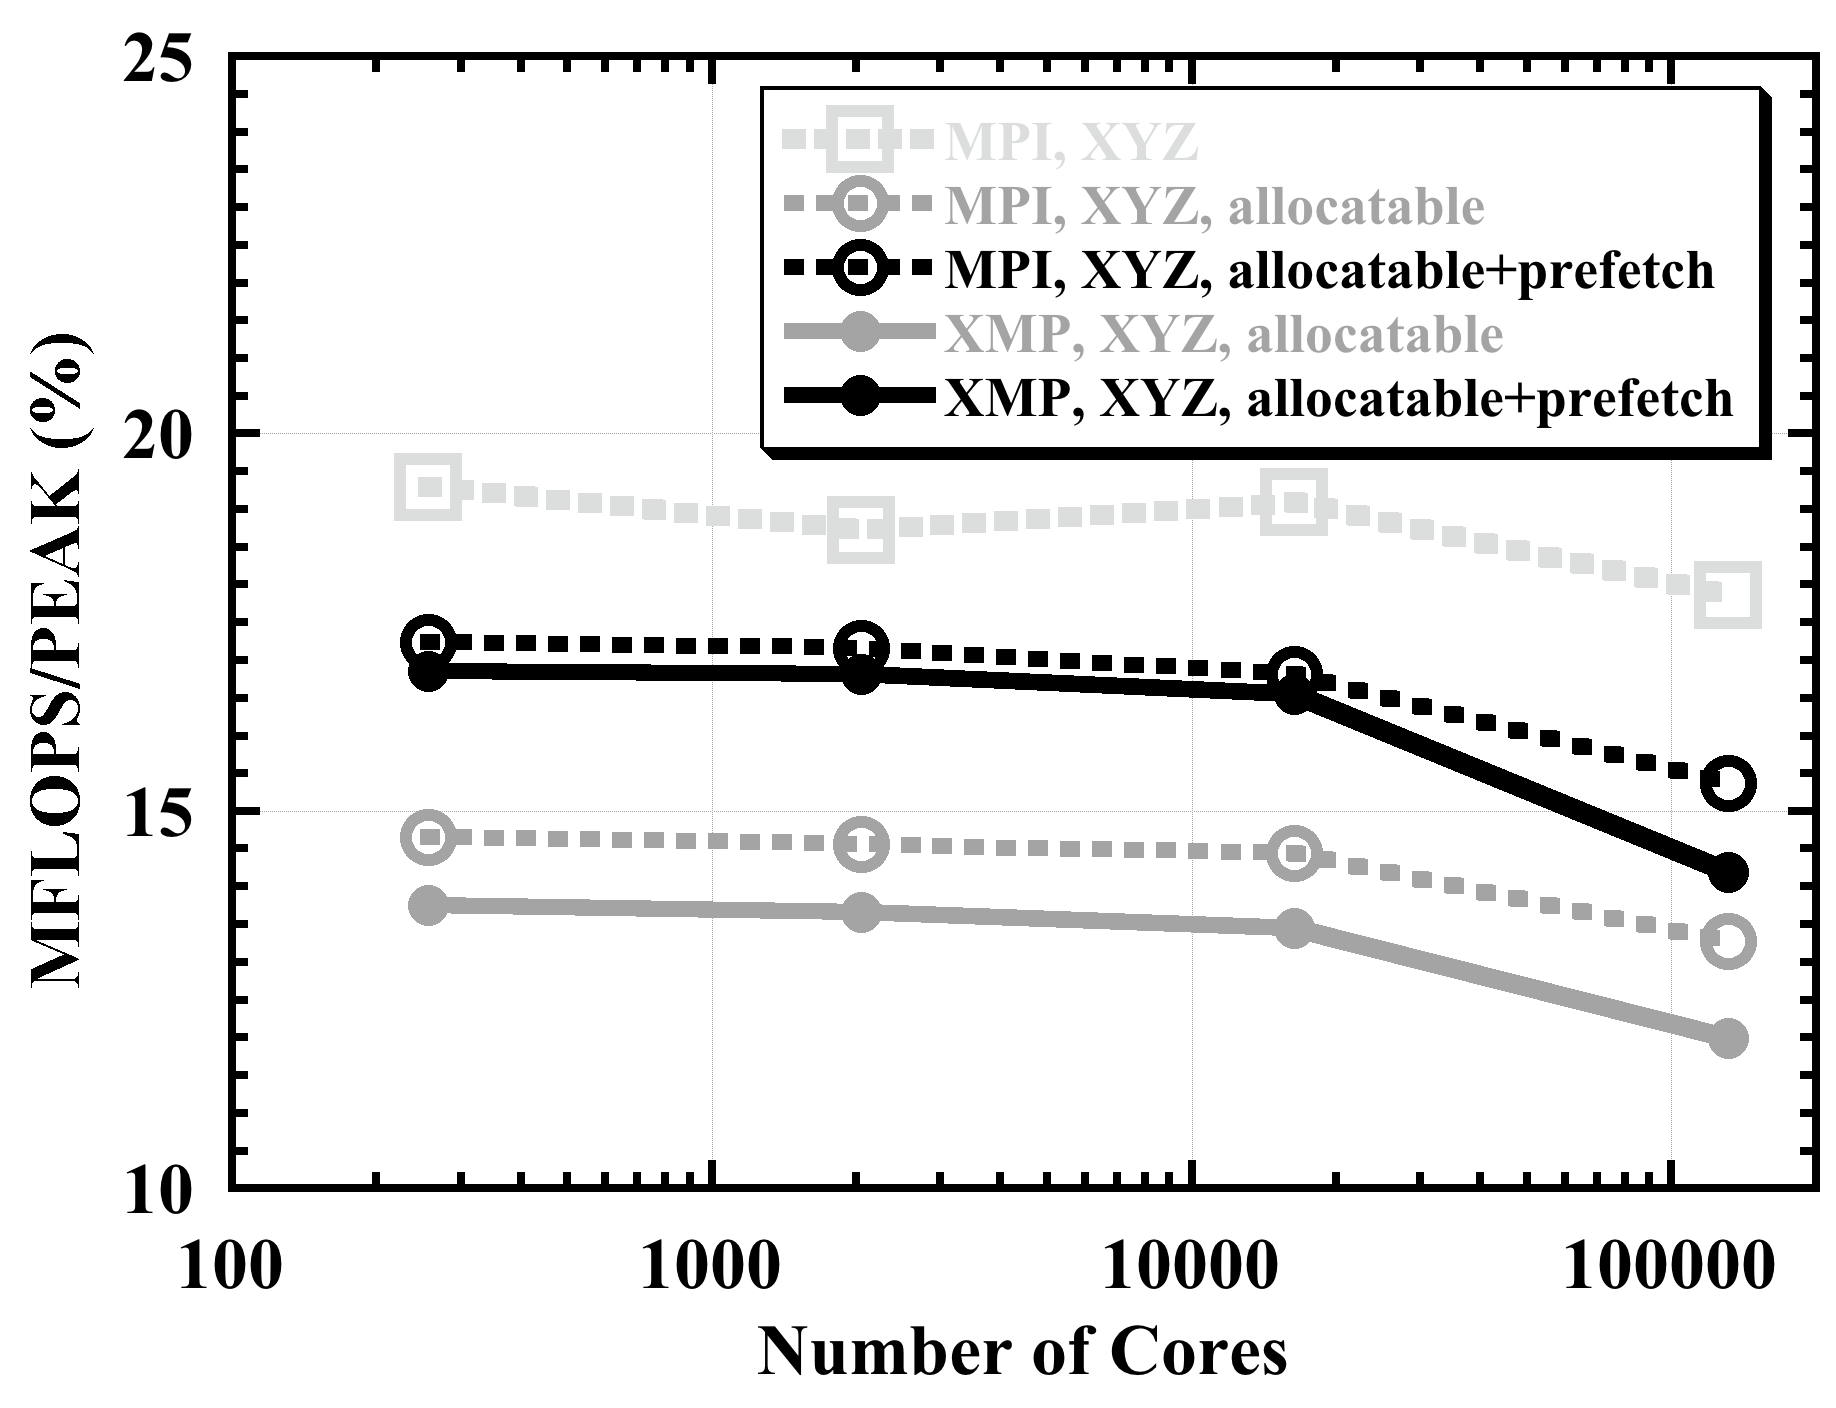
\includegraphics[width=8.5cm,bb= 0 0 459 352]{fig6-4.png}
\end{center}
\caption{IMFLOPS/PEAK measured by the hardware monitor installed on the K computer with prefetch optimization by {\it prefetch\_stride} compiler option. Solid and dash lines indicate performances of  XMP and MPI codes, respectively. Colors of light gray, gray and black indicate static arrays, allocatable arrays and allocatable arrays with prefetch optimization, respectively.}
\label{fig6-4} 
\end{figure}

MFLOPS/PEAK values are dropped from 20\% to 15\%, and this performance degradation without the prefetch instructions is confirmed. To force the native Fortran compiler to perform the prefetch optimization, we can use {\it prefetch\_stride} compiler option. All codes are recompiled with {\it prefetch\_stride} compiler option and rerun. Performance improvements by this compiler option are shown in Fig. \ref{fig6-4} for both MPI (gray dash to black dash) and XMP (gray solid to black solid) codes. MFLOPS/PEAK values are improved by 2\textasciitilde 3\% with the prefetch optimization. Finally we can get almost the same performance with XMP as that of MPI when allocatable arrays are used, but efforts to shrink the performance gap between static and allocatable arrays are still needed. 

\section{Local-view Programming Model}
In the locall-view programming model, communications among domains are written by Fortran Coarray assignment statements, with which two types of one-sided communications for local data, namely {\it put} and {\it get}, are adopted. For the sake of simplicity, we focus on the all of X, Y and Z domain decomposition method in this section.

\subsubsection{Communications using Coarray}
Just same as the MPI program, DO loop boundaries in the original source code must be modified and communications must be explicitly written 
by Coarray assignment statements. Typical XMP Fortran programs using {\it put} communications are shown in Listing \ref{local}, which is corresponding to Listing \ref{allxyz}. Division numbers are defined just as variables, not parameters to easily change them by input data without recompilations. As Coarray features in Fortran 2008, which is supported by the XMP/F compiler at that time, do not include reduction operations, the code to obtain the maximum value of the scalar variable in whole simulation system must be hand-coded. But Coarray features in Fortran 2015 support reduction operations by intrinsic subroutines, and these codes are simply replaced with {\it co\_max} intrinsic subroutine, which is shown in Listing \ref{comax}. These intrinsic subroutines are partially supported by the current XMP/F compiler.

\begin{lstlisting}[caption=Typical XMP programs using the local-view programming model with {\it put} communications for all of X{,} Y and Z domain decomposition method., label=local]
integer, parameter :: lx=..., ly=..., lz=...
real*8 :: ram
real*8, allocatable :: rami(:)
real*8, allocatable :: physval(6,:,:,:)[:]
real*8 :: ramc[*]
...
limgn = THIS_IMAGE()
lsx = lx / nx
lsy = ly / ny
lsz = lz / nz
linxp = limgn + 1
linxm = limgn - 1
linyp = limgn + nx
linym = limgn - nx
linzp = limgn + (nx*ny)
linzm = limgn - (nx*ny)
allocate( physval(6,0:lsx+1,0:lsy+1,0:lsz+1)[*] )
allocate( rami(nx*ny*nz) )
...
physval(:,lsx+1,:,:)[linxm] = physval1(:,1,:,:)
physval(:,0,:,:)[linxp] = physval1(:,lsx,:,:)
SYNC ALL
!$OMP PARALLEL DO PRIVATE(iy,ix)
do iz = 1, lsz
 do iy = 1, lsy
  do ix = 1, lsx
   ...
   physval(..,ix,iy,iz) = ... &
      physval(..,ix-1,iy,iz) ... physval(..,ix+1,iy,iz)
   ...
...
physval(:,:,lsy+1,:)[linym] = physval1(:,:,1,:)
physval(:,:,0,:)[linyp] = physval1(:,:,lsy,:)
SYNC ALL
!$OMP PARALLEL DO PRIVATE(iy,ix)
do iz = 1, lsz
 do iy = 1, lsy
  do ix = 1, lsx 
   ...
   physval(..,ix,iy,iz) = ... &
      physval(..,ix,iy-1,iz) ... physval(..,ix,iy+1,iz)
   ...
...
physval(:,:,:,lsz+1)[linzm] = physval1(:,:,:,1)
physval(:,:,:,0)[linzp] = physval1(:,:,:,lsz)
SYNC ALL
!$OMP PARALLEL DO PRIVATE(iy,ix)
do iz = 1, lsz
 do iy = 1, lsy
  do ix = 1, lsx 
   ...
   physval(..,ix,iy,iz) = ... &
      physval(..,ix,iy,iz-1) ... physval(..,ix,iy,iz+1)
   ...
...
!$OMP PARALLEL DO REDUCTION(max:ram) PRIVATE(iy,ix)
do iz = 1, lsz
 do iy = 1, lsy
  do ix = 1, lsx 
   ram = max( ram, ... )
...
ramc = ram
SYNC ALL
if( limgn .eq. 1 ) then
 rami(1) = ram
 do i = 2, nx*ny*nz
  rami(i) = ramc[i]
 end do
 ram = max( rami )
 ramc = ram
end if
SYNC ALL
if( limgn .ne. 1 ) then
 ram = ramc[1]
end if  
\end{lstlisting}

\begin{lstlisting}[caption=Reduction operations can be replaced by an intrinsic subroutine., label=comax]
...
call CO_MAX( ram ) 
...
\end{lstlisting}

Differences of programs between {\it put} and {\it get} communications are only in Coarray assignment and related {\it sync all} statements, and the other parts are completely same. Ttypical XMP Fortran programs related with {\it get} communications are shown in Listing \ref{get}. Note that related {\it sync all} statement must be written after {\it put} or before {\it get} communications.

\begin{lstlisting}[caption=Typical XMP programs using the local-view programming model with {\it get} communications for all of X{,} Y and Z domain decomposition method., label=get]
...
SYNC ALL
physval(:,lsx+1,:,:) = physval1(:,1,:,:)[linxp]
physval(:,0,:,:) = physval1(:,lsx,:,:)[linxm]
...
SYNC ALL
physval(:,:,lsy+1,:) = physval1(:,:,1,:)[linyp]
physval(:,:,0,:) = physval1(:,:,lsy,:)[linym]
...
SYNC ALL
physval(:,:,:,lsz+1)= physval1(:,:,:,1)[linzp] 
physval(:,:,:,0)= physval1(:,:,:,lsz)[linzm] 
...
\end{lstlisting}

\subsection{Performance on the K Computer}
We run three XMP codes using the global-view programming model, and the locall-view programming model with {\it put} and {\it get} communications, and local-view communications are implemented on Fujitsu RDMA. Each process performs computations with 8 threads just like before and we evaluate the weak scaling on the K computer using Omni XcalableMP 0.9.1 and Fujitsu Fortran K-1.2.0.18.
A number of cores for execution and corresponding simulation parameters are summarized in Table \ref{tab6-2} and performance are also measured by a hardware monitor installed on the K computer. As versions of both Omni XcalableMP and Fujitsu Fortran compilers are different from those of previous section, we also rerun the global-view programming model code. MFLOPS/PEAK values for all cases are shown in Fig. \ref{fig6-5}.

\begin{table}[h]
\caption{Simulation Parameters for Local-view Programming Model}
\label{tab6-2}
\begin{tabular}{p{2cm}p{2cm}p{1.5cm}p{1.5cm}p{1.5cm}}
\hline\noalign{\smallskip}
\#core & {\it lx=ly=lz} & \multicolumn{3}{l}{all of X, Y and Z} \\
\cline{3-5}
 & & {\it nx} & {\it ny} & {\it nz} \\
\noalign{\smallskip}\svhline\noalign{\smallskip}
256 & 1024 & 4 & 4 & 2 \\
2048 & 2048 & 8 & 8 & 4 \\
16384 & 4096 & 16 & 16 & 8 \\
\noalign{\smallskip}\hline\noalign{\smallskip}
\end{tabular}
\end{table}

\begin{figure}[h]
%\sidecaption
\begin{center}
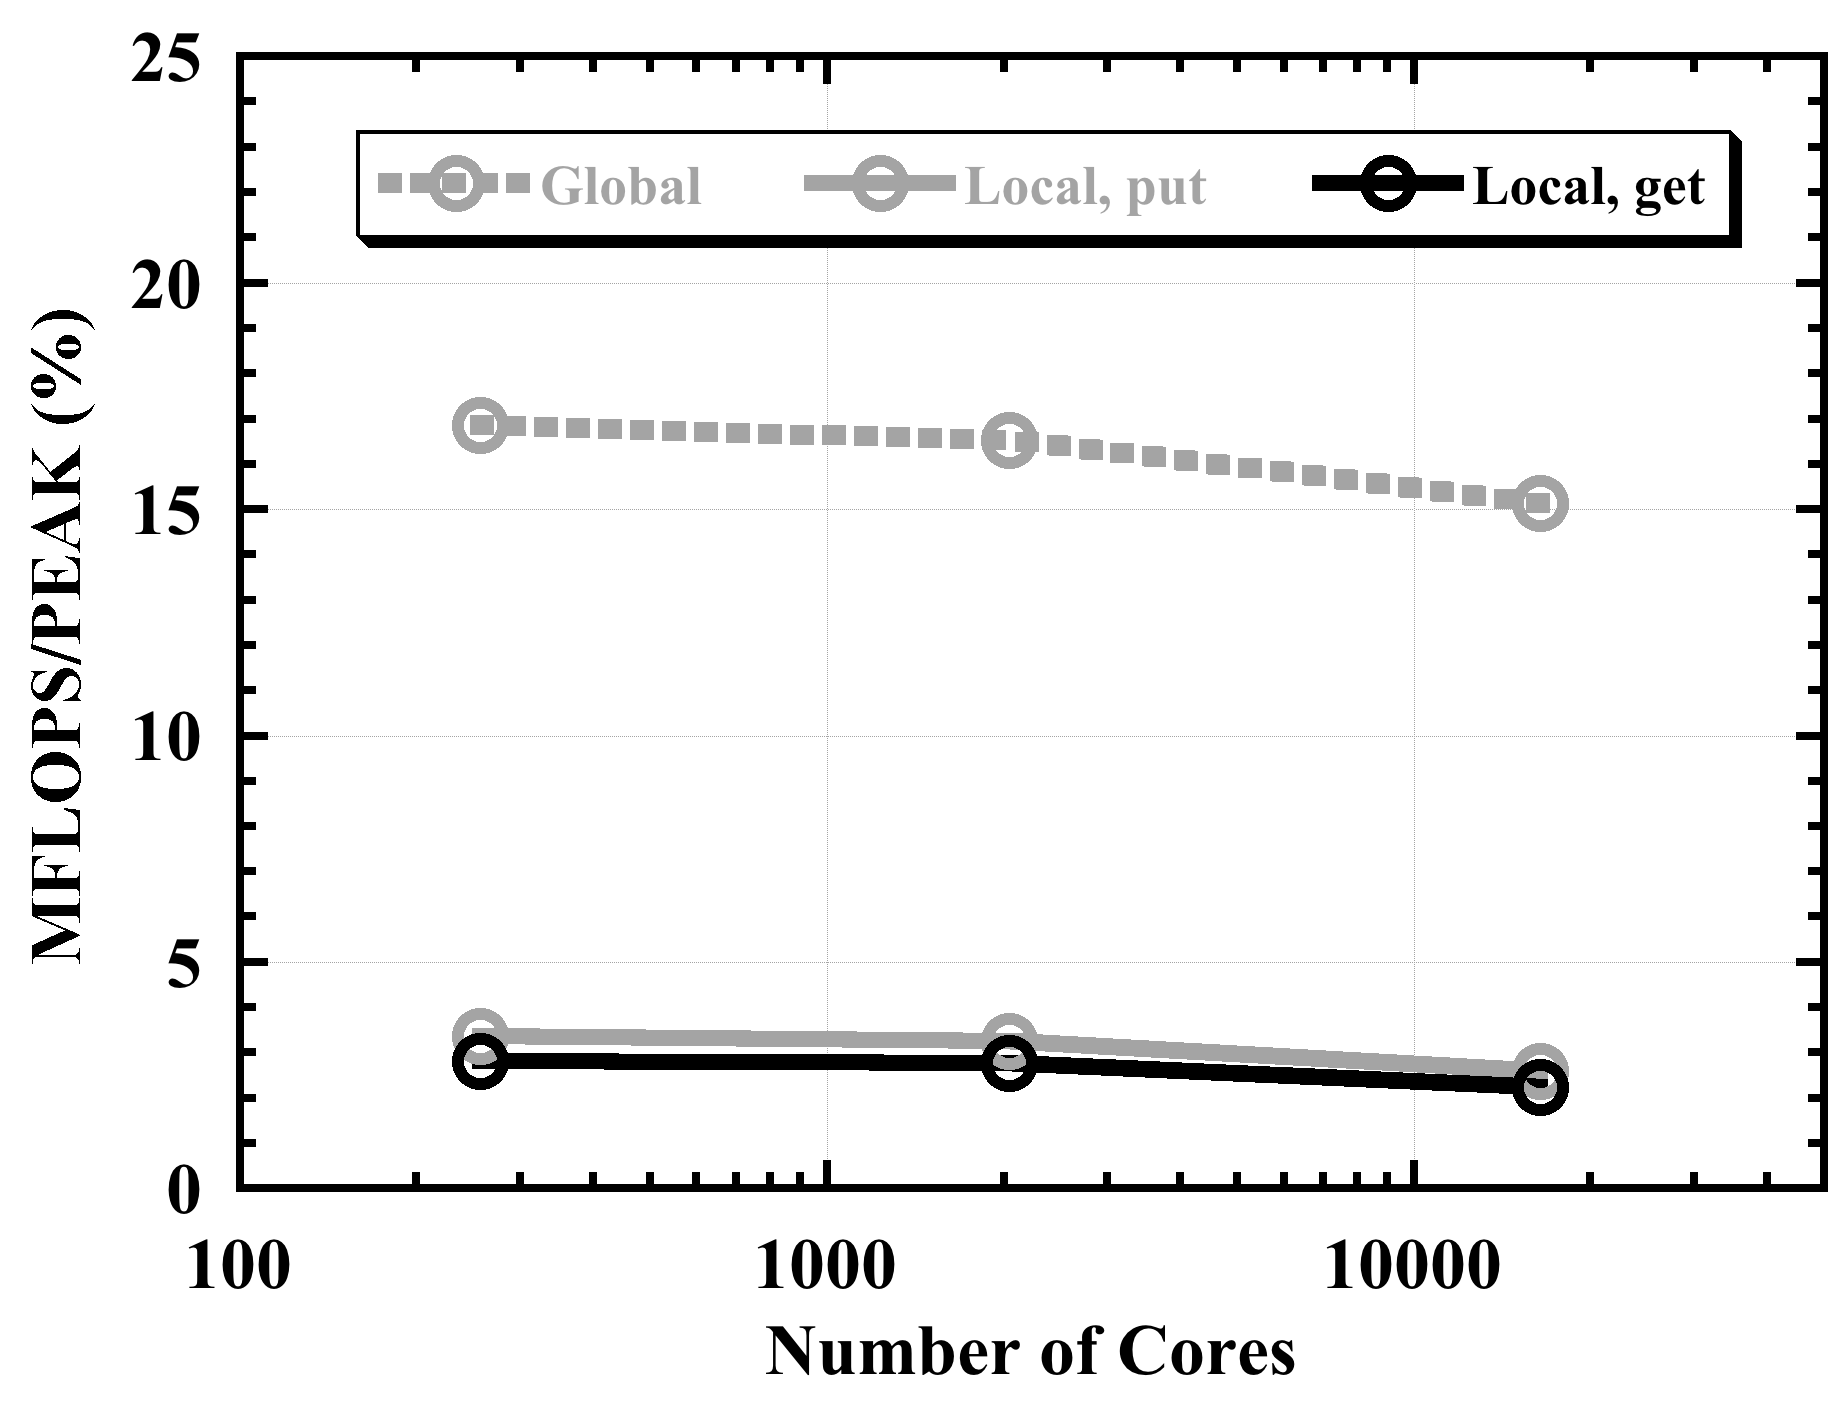
\includegraphics[width=8.5cm,bb=0 0 461 352]{fig6-5.png}
\end{center}
\caption{MFLOPS/PEAK measured by the hardware monitor installed on the K computer. Gray dash line indicates performance of the global-view programming model. Gray and black solid lines indicate performances of the local-view programming model with {\it put} and {\it get} communications, respectively.}
\label{fig6-5} 
\end{figure}

Performances using the global-view programming model are almost same as those in previous section, but the local-view programming model shows very low performances, namely 3\% of peak performance of the K computer. From the hardware monitor, we found that SIMD execution usage was less than 0.2\% in local-view programming model cases, this means that cost intensive DO loops in IMPACT-3D are not SIMDized at all even with {\it simd=2} and {\it prefetch\_stride} native Fortran compiler options. All Fortran allocatable coarrays in the local-view programming model codes are converted to pointer arrays by the XMP/F compiler. The pointer array prevents the native Fortran compiler from SIMDizing the DO loop even it is forced to SIMDize the loop by {\it simd=2} compiler option because the compiler thinks that variables may be overlapped and SIMD execution causes incorrect calculations. To tell the compiler that variables are not overlapped, we can specify {\it noalias} option and SIMD execution usage is improved to 15\%. But prefetch instructions are still suppressed and the pointer array may prevent other compiler optimizations, performances are not improved at all.

\section{Summary}
We have parallelized a three-dimensional fluid code with XMP Fortran using the global-view programming model and compared XMP performances with those of the hand-coded MPI program on the K computer. We found that performances of XMP programs are as same as those of MPI programs but these are only 8\textasciitilde 9\% of peak performance of the K computer. It was found that this relative low performance is due to lack of SIMD execution according to SIMD execution usage by the hardware monitor. We forced the native Fortran compiler to SIMDize loops with the specific compiler option, and found that performance of MPI programs reach to 20\% of peak performance even those of XMP programs remain around 15\%. It was found that this relative low performance is due to low memory throughput according to Memory throughput/PEAK by the hardware monitor. Finally we could get almost the same performance of XMP codes as those of MPI codes by using additional specific compiler option of the native Fortran compiler. 

Next we parallelized the code using the local-view programming model, and also measured its performance on the K computer. We found that translated programs prevent SIMDization by the native Fortran compiler and show only 3\% of peak performance of the K computer, much lower performance than that of the global-view programming model programs. This degradation can not be solved by simply specifying native compiler options at this moment, and improvements of the XMP/F compiler are expected.

These kinds of advanced performance optimization techniques of the native Fortran compiler are not clear and may be somewhat difficult for computational scientists, but XMP programming still requires much less efforts than those for MPI programming.

\acknowledgement{This work was partially supported by JSPS Grant-in-Aid for Scientific Research (C)(25400539). Part of the research was funded by MEXT’s program for the Development and Improvement for the Next Generation Ultra High-Speed Computer System, under its Subsidies for Operating the Specific Advanced Large Research Facilities.}

%%%%%%%%%%%%%%%%%%%%%%%% referenc.tex %%%%%%%%%%%%%%%%%%%%%%%%%%%%%%
% sample references
% %
% Use this file as a template for your own input.
%
%%%%%%%%%%%%%%%%%%%%%%%% Springer-Verlag %%%%%%%%%%%%%%%%%%%%%%%%%%
%
% BibTeX users please use
% \bibliographystyle{}
% \bibliography{}
%
\begin{thebibliography}{99.}%
% Online Document
%\bibitem{phys-online} J. Dod, in \textit{The Dictionary of Substances and Their Effects}, Royal Society of Chemistry. (Available via DIALOG, 1999), 
%\url{http://www.rsc.org/dose/title of subordinate document. Cited 15 Jan 1999}
%
% Monograph
%\bibitem{phys-mono} H. Ibach, H. L\"uth, \textit{Solid-State Physics}, 2nd edn. (Springer, New York, 1996), pp. 45-56 
%
% Journal article
%\bibitem{phys-journal} S. Preuss, A. Demchuk Jr., M. Stuke, Appl. Phys. A \textbf{61}
%
% Journal article by DOI
%\bibitem{phys-DOI} M.K. Slifka, J.L. Whitton, J. Mol. Med., doi: 10.1007/s001090000086
%
% Contribution 
%\bibitem{phys-contrib} S.E. Smith, in \textit{Neuromuscular Junction}, ed. by E. Zaimis. Handbook of Experimental Pharmacology, vol 42 (Springer, Heidelberg, 1976), p. 593
%
\bibitem{XMP} XcalableMP, \url{http://www.xcalablemp.org/}.

\bibitem{Omni} Omni XMP compiler, \url{http://omni-compiler.org/xcalablemp.html}.

\bibitem{HPF} High Performance Fortran, \url{http://hpff.rice.edu/}.

\bibitem{Ken} K. Kennedy, C. Koelbel, H. Zima, Proc. 3rd ACM SIGPLAN conference on History of programming languages, pp.7-1-7-22 (2007).

\bibitem{Zhang} Y. Zhang, H. Iwashita, K. Ishii, M. Kaneko, T. Nakamura, K. Hotta, Proc. 6th Int. Workshop on OpenMP, pp.133-148 (2010).

\bibitem{CAF} J. Reid, {\it Coarrays in the next Fortran Standard}, ISO/IEC JTC1/SC22/WG5 N1787 (2009).

\bibitem{SC02} H. Sakagami, H. Murai, Y. Seo, M. Yokokawa, IEEE/ACM SC2002 Conference, pap147 (2002).

\end{thebibliography}


\end{document}
